\chapter{METHODOLOGY}
{\baselineskip=2\baselineskip
	
This chapter presents the research methodology used in the study, it covers the in-depth details of the procedures and steps taken in the research design, design procedure, system development, and deployment process of this study.


\section { System Architecture}

\begin{figure}[h]
	\centering
	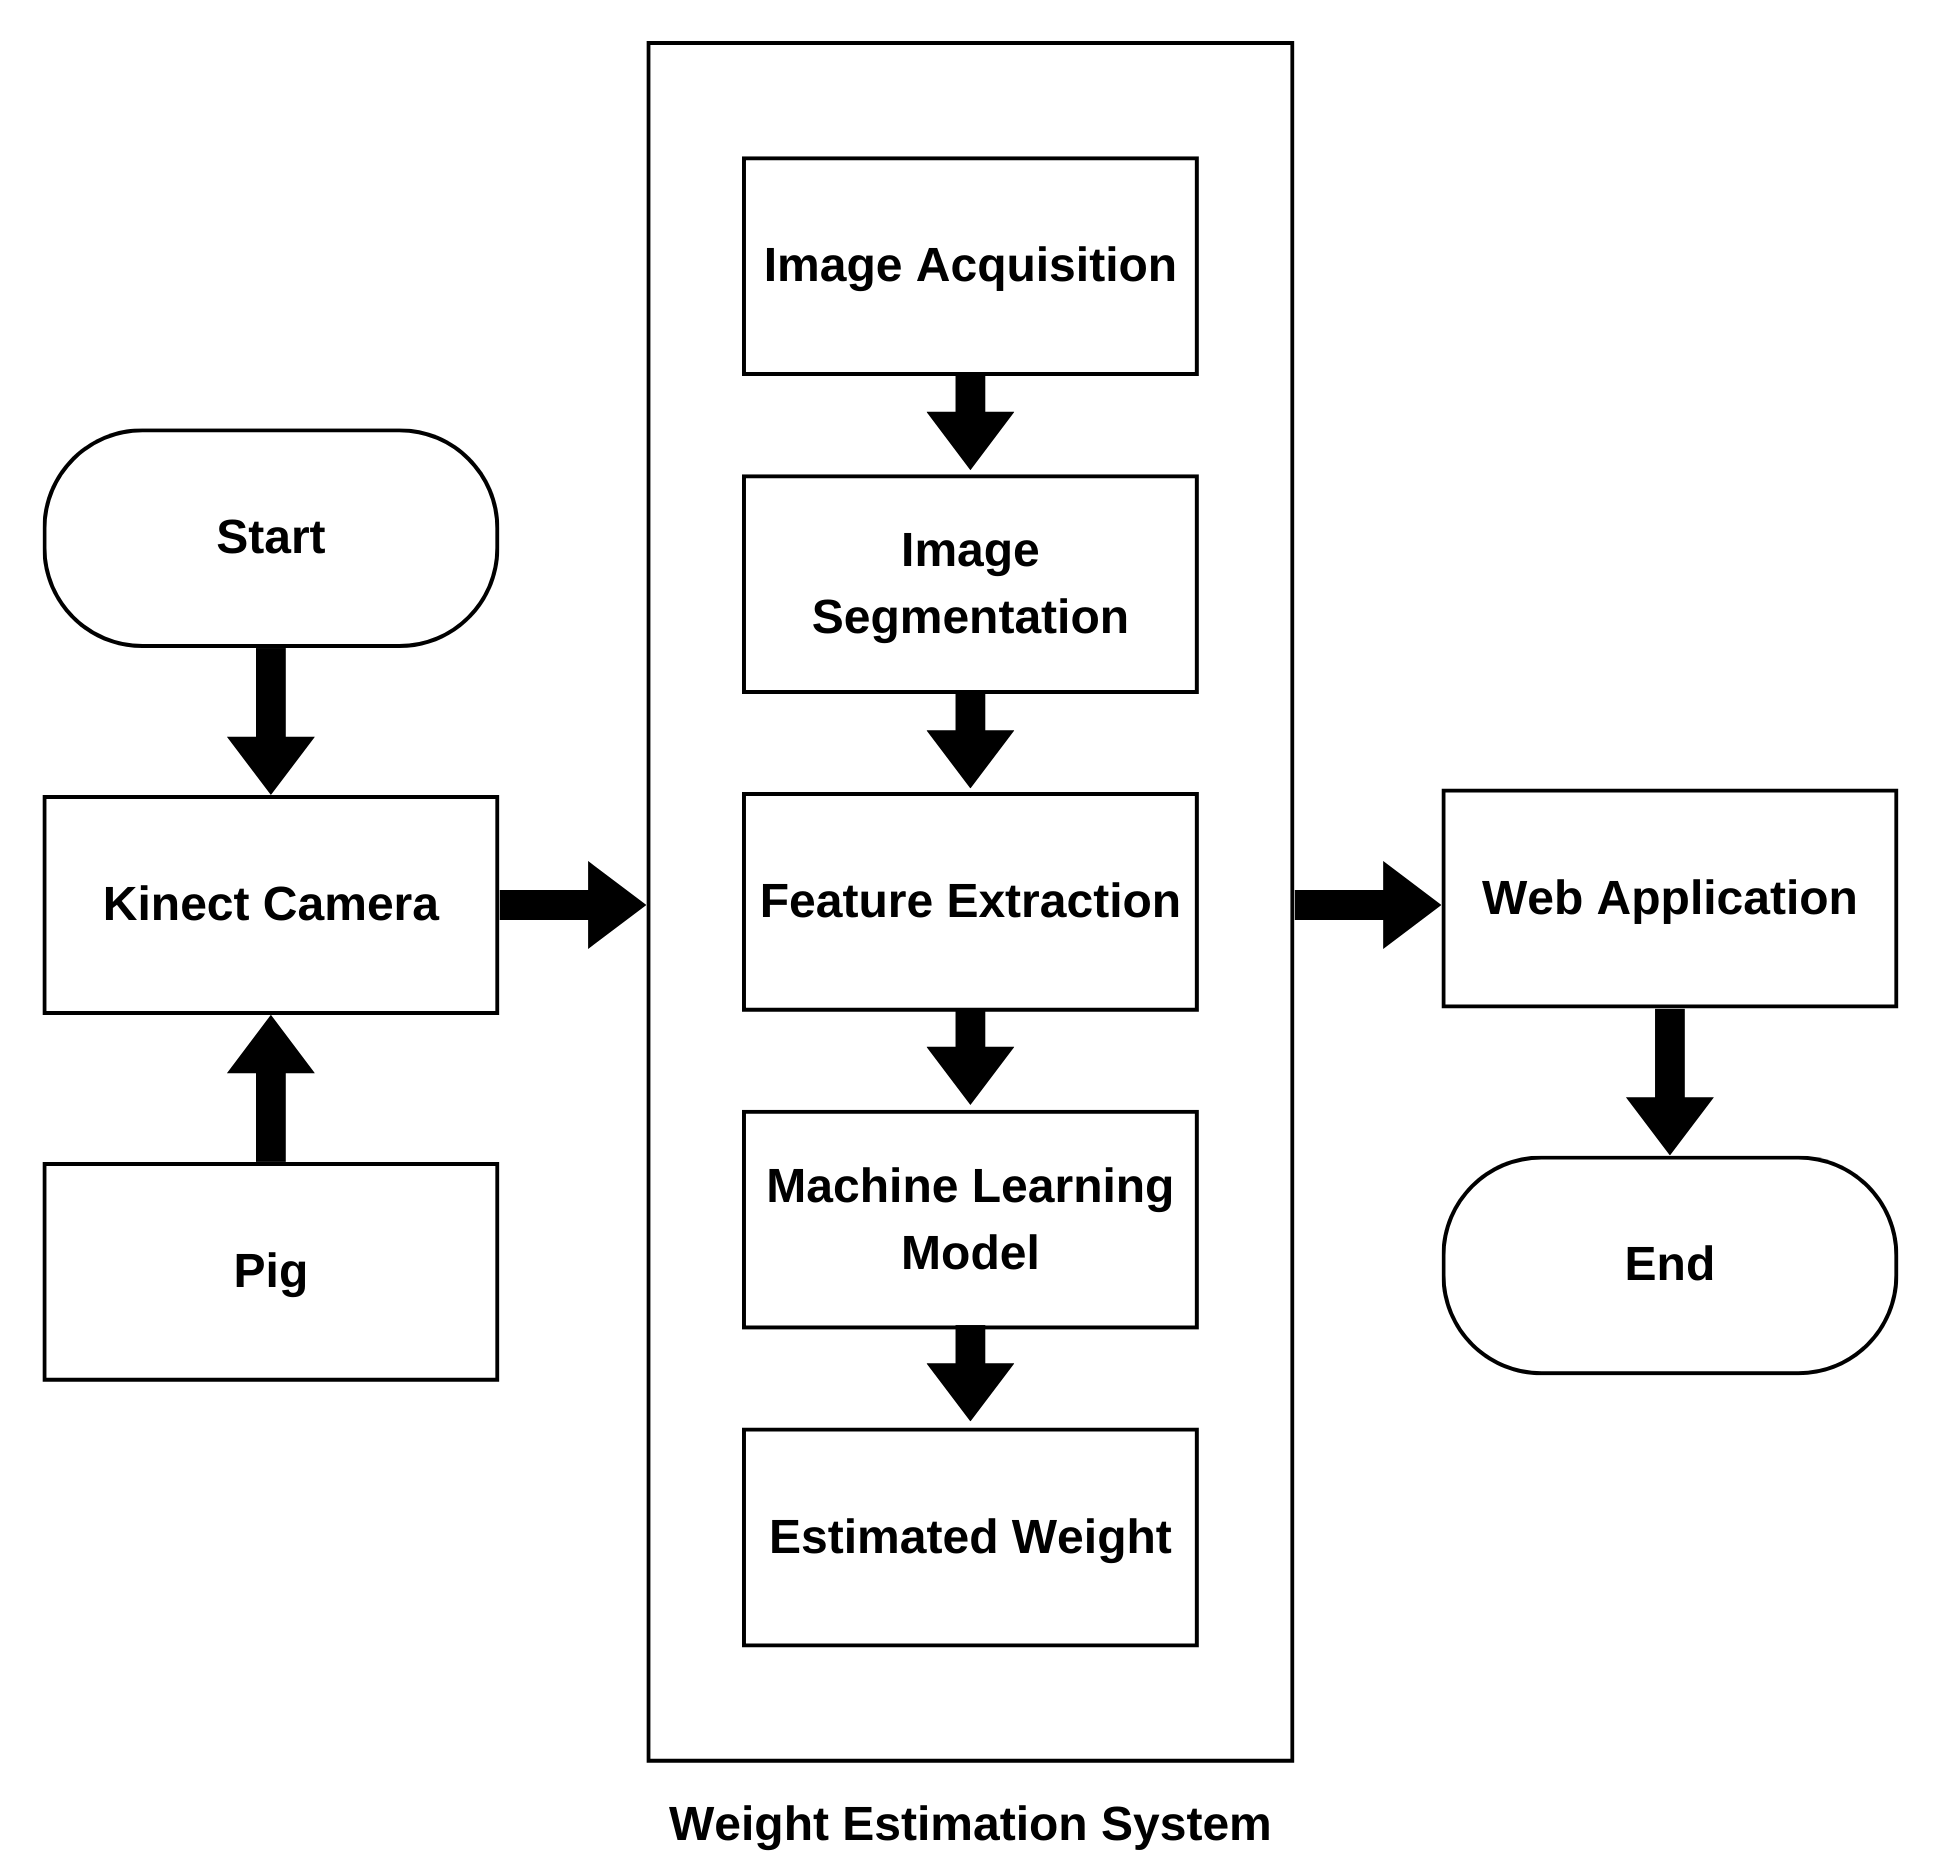
\includegraphics[height=0.4\textheight]{figures/Architectureofniggas}
	\caption{}
	\label{fig:System Architecture}
\end{figure}

Figure 1 shows the system architecture of the pig weight estimation system. It consists of the pig to be captured, the Kinect camera that will be used for taking depth images, and the system for the processing of all the data. A laptop will be used for the processing of data, which will include the processing of images, extraction of pig’s features, and calculation of estimated weight with a machine learning model. The result can then be accessed in a web application, where actual and estimated weights can be validated.

\subsection { Waterfall Model}
\begin{figure}[h]
	\centering
	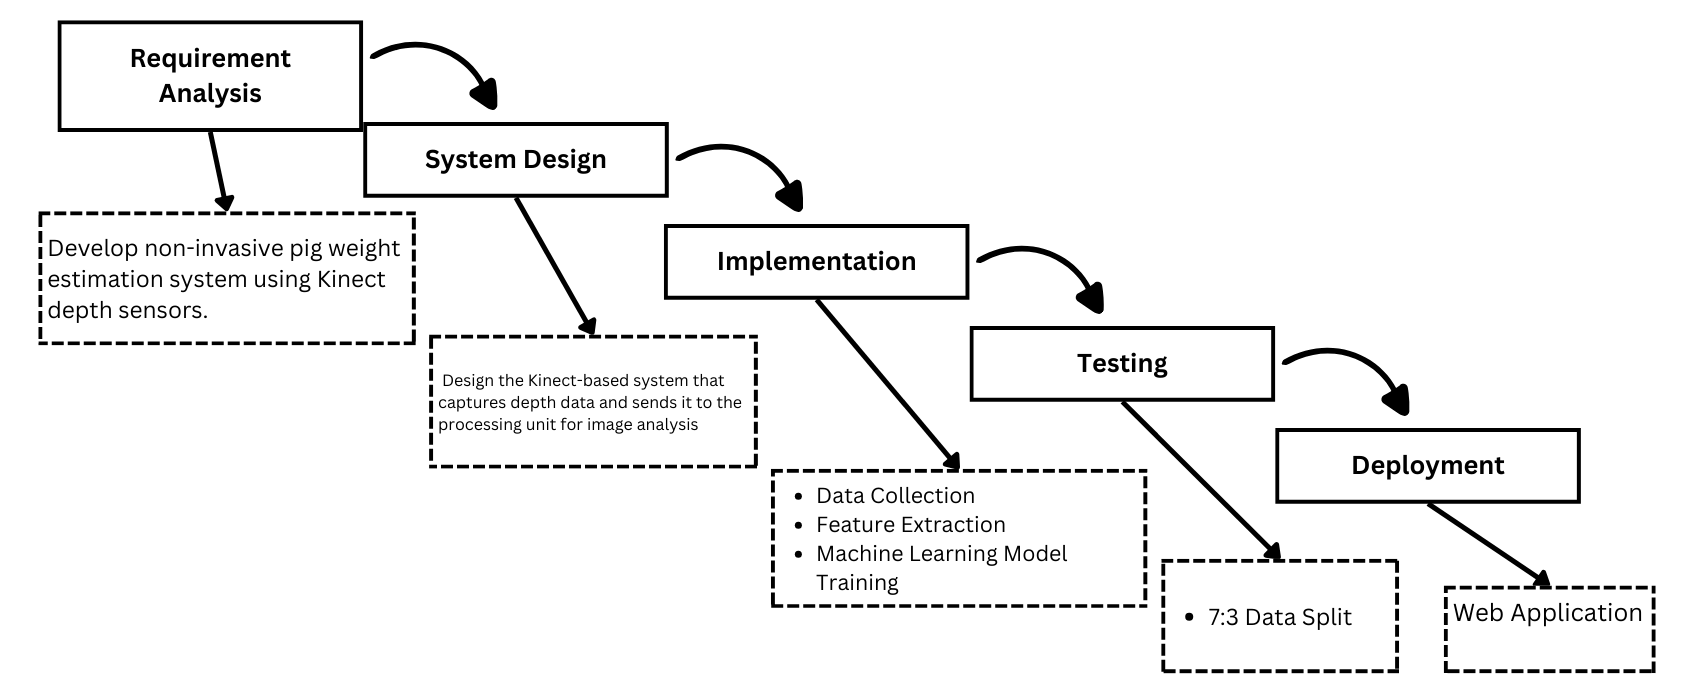
\includegraphics[height=0.4\textheight]{figures/Requirement Analysis (4)}
	\caption{}
	\label{fig:Waterfall Model}
\end{figure}

Figure 2 shows the Waterfall Model of the Weight Estimation System. Requirement Analysis, defines the goal for creating a non-invasive pig weight estimation system using a Kinect depth sensor. The system captures depth images, extracts features like height and volume, and predicts weight through machine learning models, with results available via a web app. System Design plans the architecture, including hardware and software components. For the hardware components, a Kinect sensor, a computer system, and a pig pen setup are required. While a Machine learning model and a web application is required for the software components. Implementation involves collecting images, extracting features, and training machine learning models. The Kinect sensor gathers the images to be processed. An algorithm extracts the features such as the height, area and volume from the depth images. The image processing involves grayscale conversion of the gathered images, contour detection and feature segmentation to isolate pig features. The training of the machine learning model follows a ratio of 7:3 for the training data and the testing data respectively. The testing phase assesses the system's accuracy using performance metrics such as MAE and RMSE. Following the 7:3 ratio, 30 percent of the gathered data set is used in the testing of the machine learning models in which the most accurate model is selected. The system is deployed using a web application that displays the weight estimates based on input depths.
\newpage
\subsection {Flowchart}
\begin{figure}[h]
	\centering
	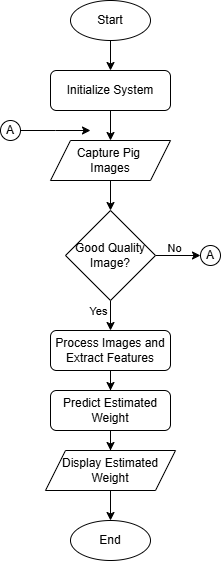
\includegraphics[height=0.6\textheight]{figures/kinectpigNIGGA}
	\caption{}
	\label{fig:Flowchart}
\end{figure}

Figure 3 outlines the flowchart of the weight estimation system. The process begins with system initialization, where the Kinect camera and other equipment are powered on, and the pig is prepared for imaging. Images are captured using the Kinect camera, and a good quality image is defined as clear, well-lit, free of motion blur, and accurately representing the pig's dimensions. To select the highest quality image, a max voting ensemble algorithm evaluates multiple captured images based on metrics like sharpness, contrast, and brightness (Gonzalez and Woods, 2018). If no satisfactory image is found, additional captures are made until a quality image is obtained. Once a high-quality image is secured, the system moves on to image preprocessing and feature extraction, leading to the prediction of the estimated weight. The final result is then displayed in a web application for user access.
\subsection {Pigpen Diagram}

\begin{figure}[h]
	\centering
	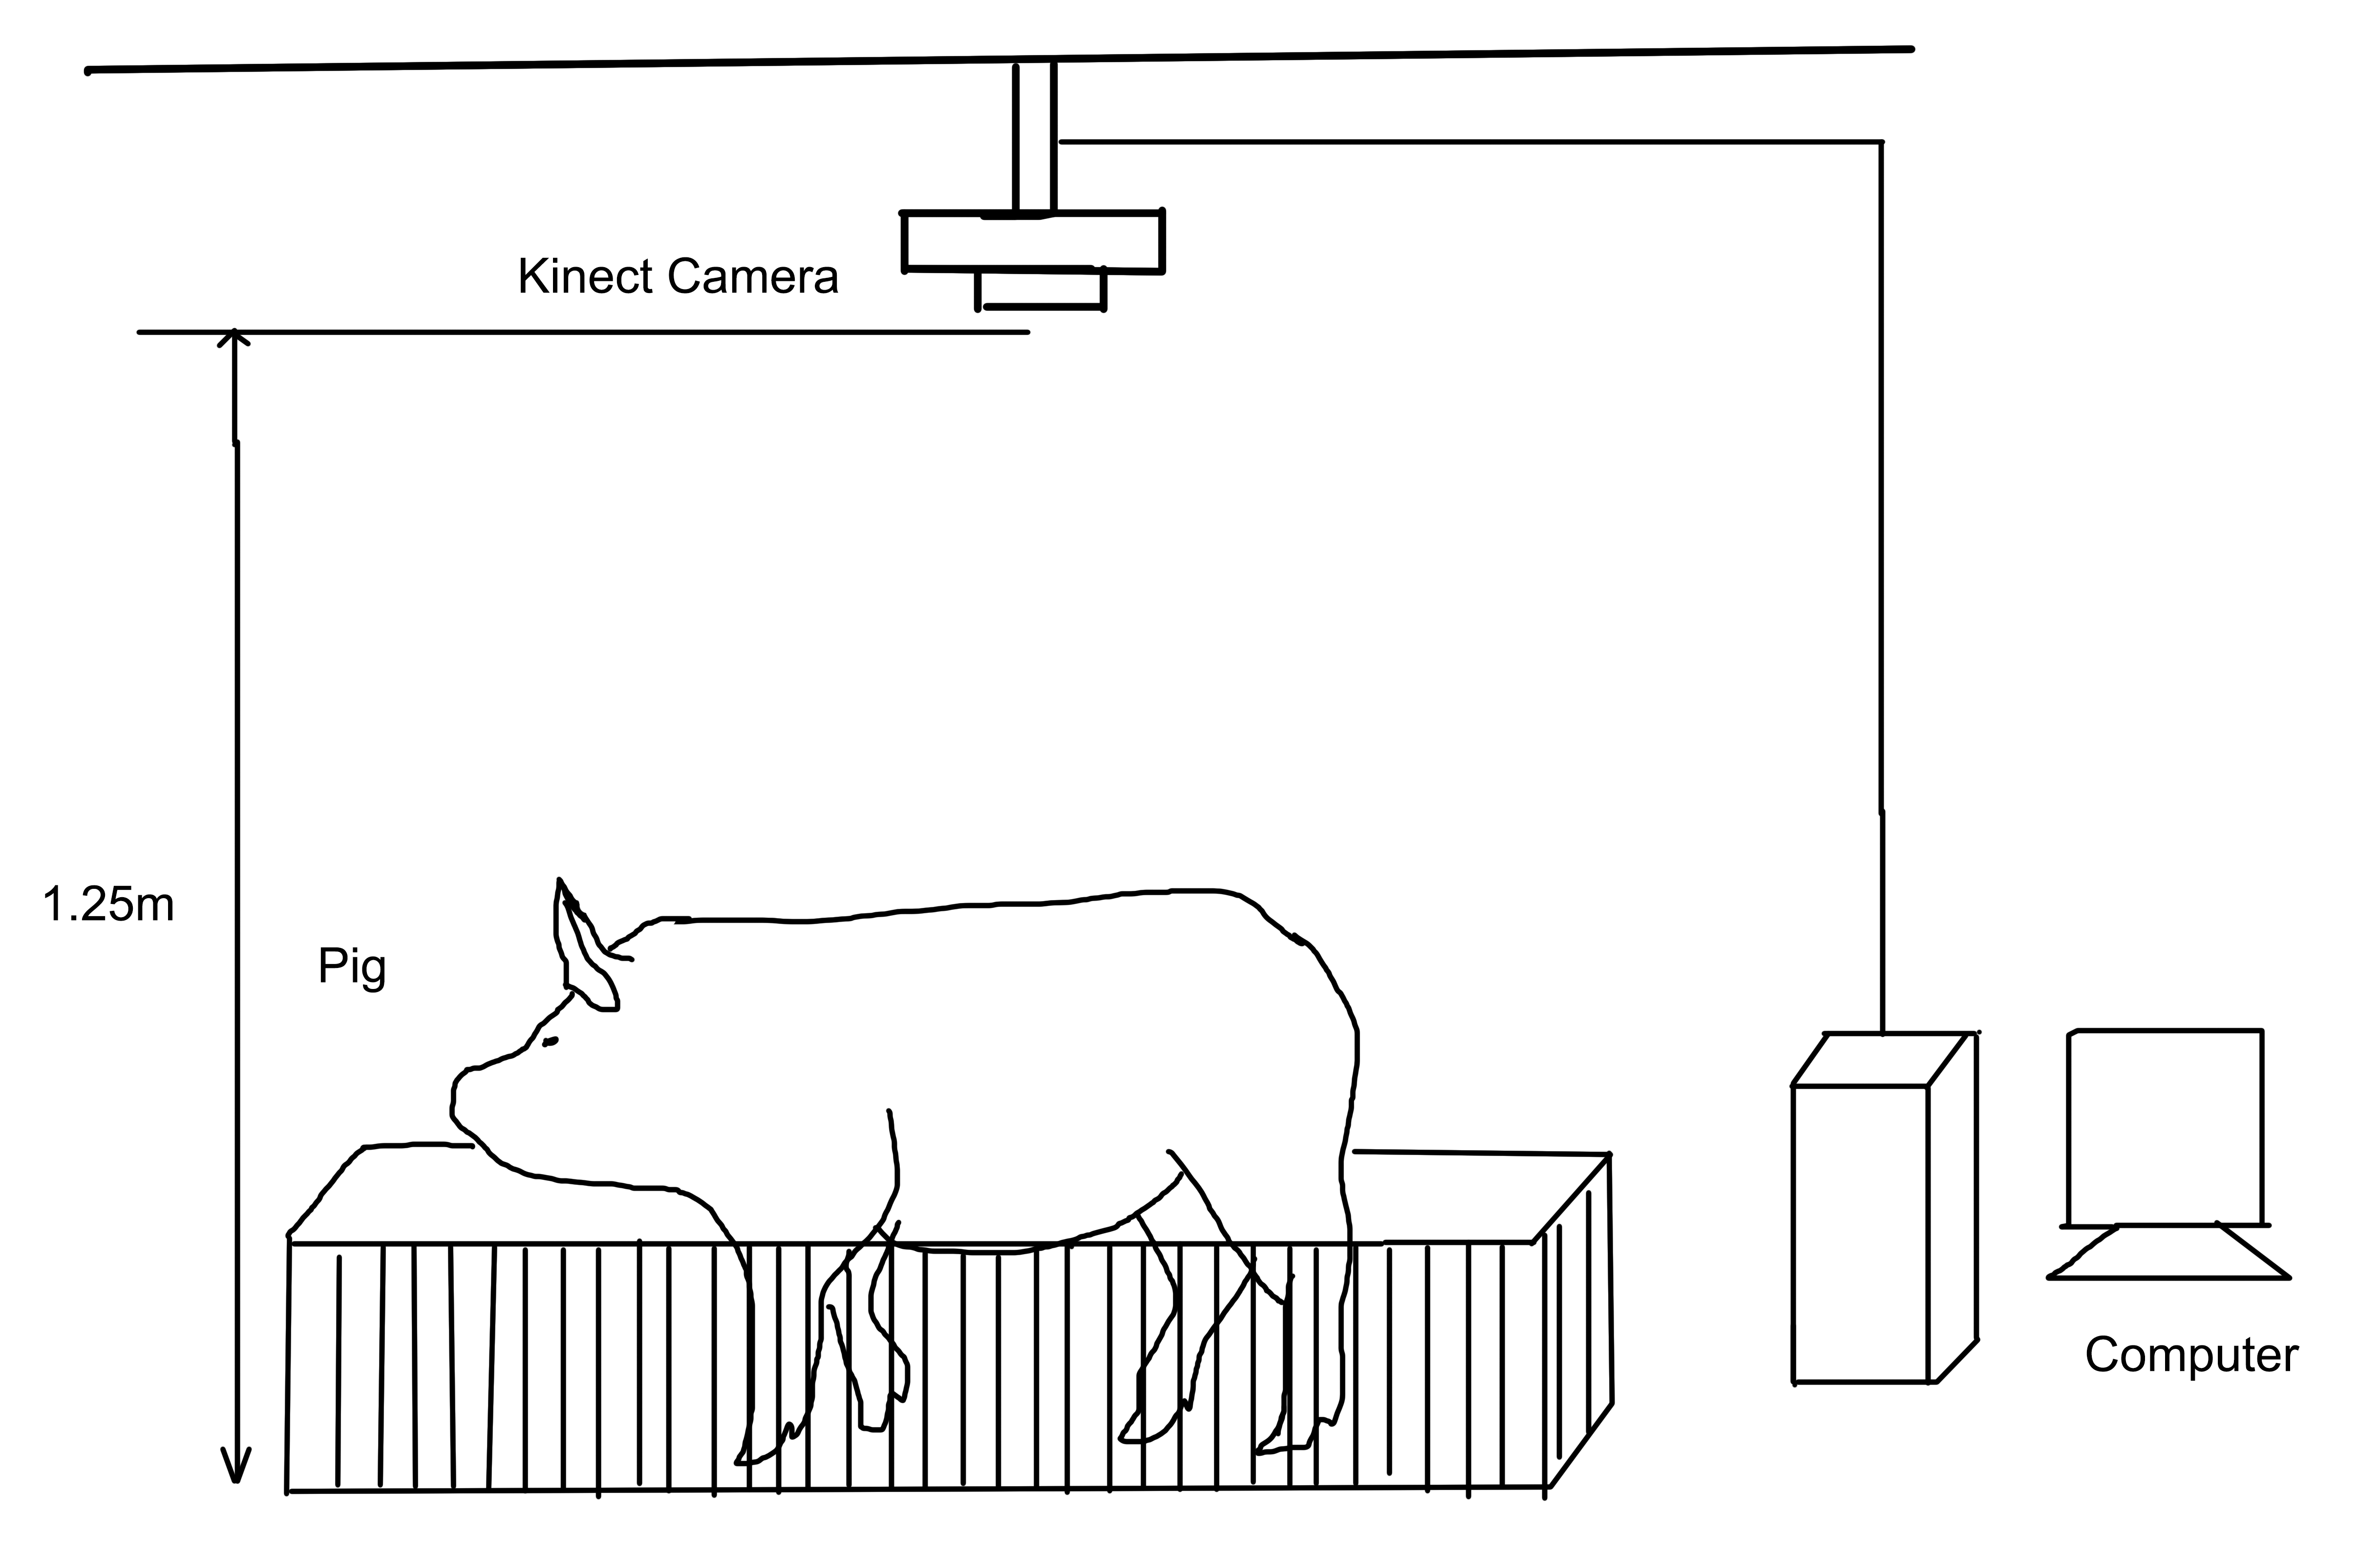
\includegraphics[height=0.4\textheight]{figures/Untitled-1wqw}
	\caption{}
	\label{fig:Pigpen Diagram}
\end{figure}

Figure 4 presents a diagram of the pigpen, illustrating the positioning of the Kinect camera. The camera is strategically suspended 1.25 meters above the ground. This height ensures a clear capture of the pig within the pen, while remaining low enough to minimize the likelihood of capturing workers as they move around the area. Additionally, this positioning keeps the camera within its optimal range of 2 meters, maximizing its effectiveness for monitoring purposes.

\section{Study Design and Data Collection}
The study will be conducted in commercial pig weaning farms located in Northern Mindanao, Philippines, focusing on pigs of the Landrace breed. These pigs, with an average live weight ranging from 40 to 100 kilograms, are fed using commercial dry pellet feed and have access to water through standard feeders in the weaning pens. Data collection will take place within these farms, where depth images of the pigs will be captured using the Kinect V1 camera. The camera will record depth data, essential for calculating the distance between the sensor and the top of the pig, and between the sensor and the ground. This is needed for the calculation of the height of the pig, which will be used to estimate the pig's weight.
Several environmental factors will also be monitored during data collection, such as lighting conditions and temperature. The size of the pen in the weaning barn will be recorded to ensure consistent environmental conditions for all pigs observed. Additionally, the temperature of the area during observation will be measured, as fluctuations in temperature can influence the pigs’ behavior and posture. The lighting conditions within the observation area will also be documented, given that lighting can impact the quality of the depth images captured by the Kinect sensor. By controlling and documenting these variables, the study aims to minimize external factors that could affect the accuracy of the weight estimation model.

\section{Object Detection}
Object detection in this study isolates the pig within each frame using depth images from Kinect sensors to identify the region of interest (ROI). We employ YOLOv5 (You Only Look Once, version 5), a single-shot object detection model known for its high efficiency and accuracy in real-time applications (Bochkovskiy et al., 2020). With a CNN-based architecture, YOLOv5 processes entire images in a single pass, which optimizes speed and accuracy—key factors for agricultural use (Redmon and Farhadi, 2016; Jocher, 2021). This version was chosen over zero-shot and multi-stage detectors due to its consistent performance in detecting complex, variable shapes like animals. A pre trained YOLOv5 model, trained on Microsoft’s COCO dataset, was selected to leverage transfer learning, enabling robust adaptation to pig detection without extensive retraining (Lin et al., 2014; Howard et al., 2018). By adopting this approach, we reduce training overhead and improve detection reliability, making YOLOv5 ideal for our farm setting.

\section{Segmentation Model}
This study employs the Segmentation Anything Model (SAM) to achieve precise segmentation of the pig within the detected ROI. SAM is uniquely suited for this task due to its prompt-based, generalizable approach, which allows for accurate segmentation with minimal retraining (Kirillov et al., 2023). SAM’s adaptability is essential in agricultural settings, where it reliably captures complex shapes and contours, ensuring high-quality feature extraction of key metrics like height and area. By using SAM, we enhance the segmentation accuracy and efficiency, enabling more consistent and precise data for weight estimation.
\subsection{Image Preprocessing}
During the preprocessing stage, the image is converted to grayscale and resized. If its dimensions are smaller than the target size, symmetric padding is applied to ensure the entire pig is visible within the frame. Next, a Gaussian blur with a kernel size of (13,13) is applied; this kernel size is chosen arbitrarily to balance blurring and detail preservation. The blurred image is then subtracted from the original to enhance edges, expressed as follows:

\myequation{}
\begin{equation}
	I_{\text{sharp}}(x, y) = I(x, y) + \alpha (I(x, y) - I_{\text{blur}}(x, y))
\end{equation}

where I(x,y) is the original intensity and Iblur(x,y) is the blurred intensity. A threshold value of T=5 is chosen for binarization to effectively distinguish the pig’s silhouette from the background; this value is determined based on preliminary testing to optimize contrast without losing important details. This preprocessing workflow ensures a standardized input for subsequent models, facilitating accurate feature extraction.

\subsection{Slicing the Image}
The image is split into upper and lower halves based on the principal direction of the pig’s body. This is achieved using the eigenvalue decomposition of the covariance matrix derived from the contour points of the pig. First, the centroid of the contour is calculated using the image moments:

\myequation{}
\begin{equation}
	cX = \frac{M_{10}}{M_{00}}, \quad cY = \frac{M_{01}}{M_{00}}
\end{equation}

Where $M_00$ is the area of the contour, and$M_10$, $M_01$ are the first-order moments along with the x and y axes, respectively.
The covariance matrix $\sigma$ of the contour points is then computed as:

\myequation{}
\begin{equation}
	\Sigma = \frac{1}{N} \sum_{i=1}^{N} (p_i - \mu)(p_i - \mu)^T
\end{equation}

Where $p_1$ represents a contour point, $\mu$ is the mean of the contour points, and N is the total number of points. The eigenvector corresponding to the largest eigenvalue defines the primary direction along which the image is sliced. The eigenvector, $v=[v_x, v_y]^T$ , is used to define the slope of the line that divides the pig into upper and lower halves:

\myequation{}
\begin{equation}
	y_line(x)=\frac{v_y}{v_x} (x-cX) + cY
\end{equation}

After slicing, gaps in the binary mask are filled using a morphological closing operation. This ensures that the segmentation is continuous, filling any small holes that might have been created during slicing.

\myequation{}
\begin{equation}
	I_{\text{filled}} = I_{\text{mask}} \oplus K
\end{equation}

where K is a kernel of size (5,5) used for morphological closing.

\subsection{Valley Detection}
To segment the pig into distinct anatomical regions (head, body, legs), we detect valleys along the contour. Valleys correspond to local minima in the pig’s contour, typically where the legs meet the body or the neck separates the head from the shoulders.
First, we extract the outline of the pig and smooth the contour using linear interpolation. The interpolated contour points are then analyzed using peak detection on the inverted y-coordinates to find the valleys, representing the points of maximum curvature.
let ${(x_i, y_i)}^N _i=1$ represent the sorted interpolated contour points. The valleys are found by identifying the local maxima in the inverted contour:

\myequation{}
\begin{equation}
	v_i=arg max(-y(x))
\end{equation}

The detected valleys are sorted based on their xxx-coordinates to establish the segmentation boundaries.

\subsection{Segmentation into Sections}
Using the detected valleys, we define four primary sections: legs, body, shoulders, head. Each section is extracted by crearing binary masks between consecutive valleys:

\myequation{}
\begin{equation}
	S_region (x,y) = I_sharp (x,y) (1_[x_start,x_end])
\end{equation}

where $S_region$ is the segmented region of interest.

\begin{figure}[h]
	\centering
	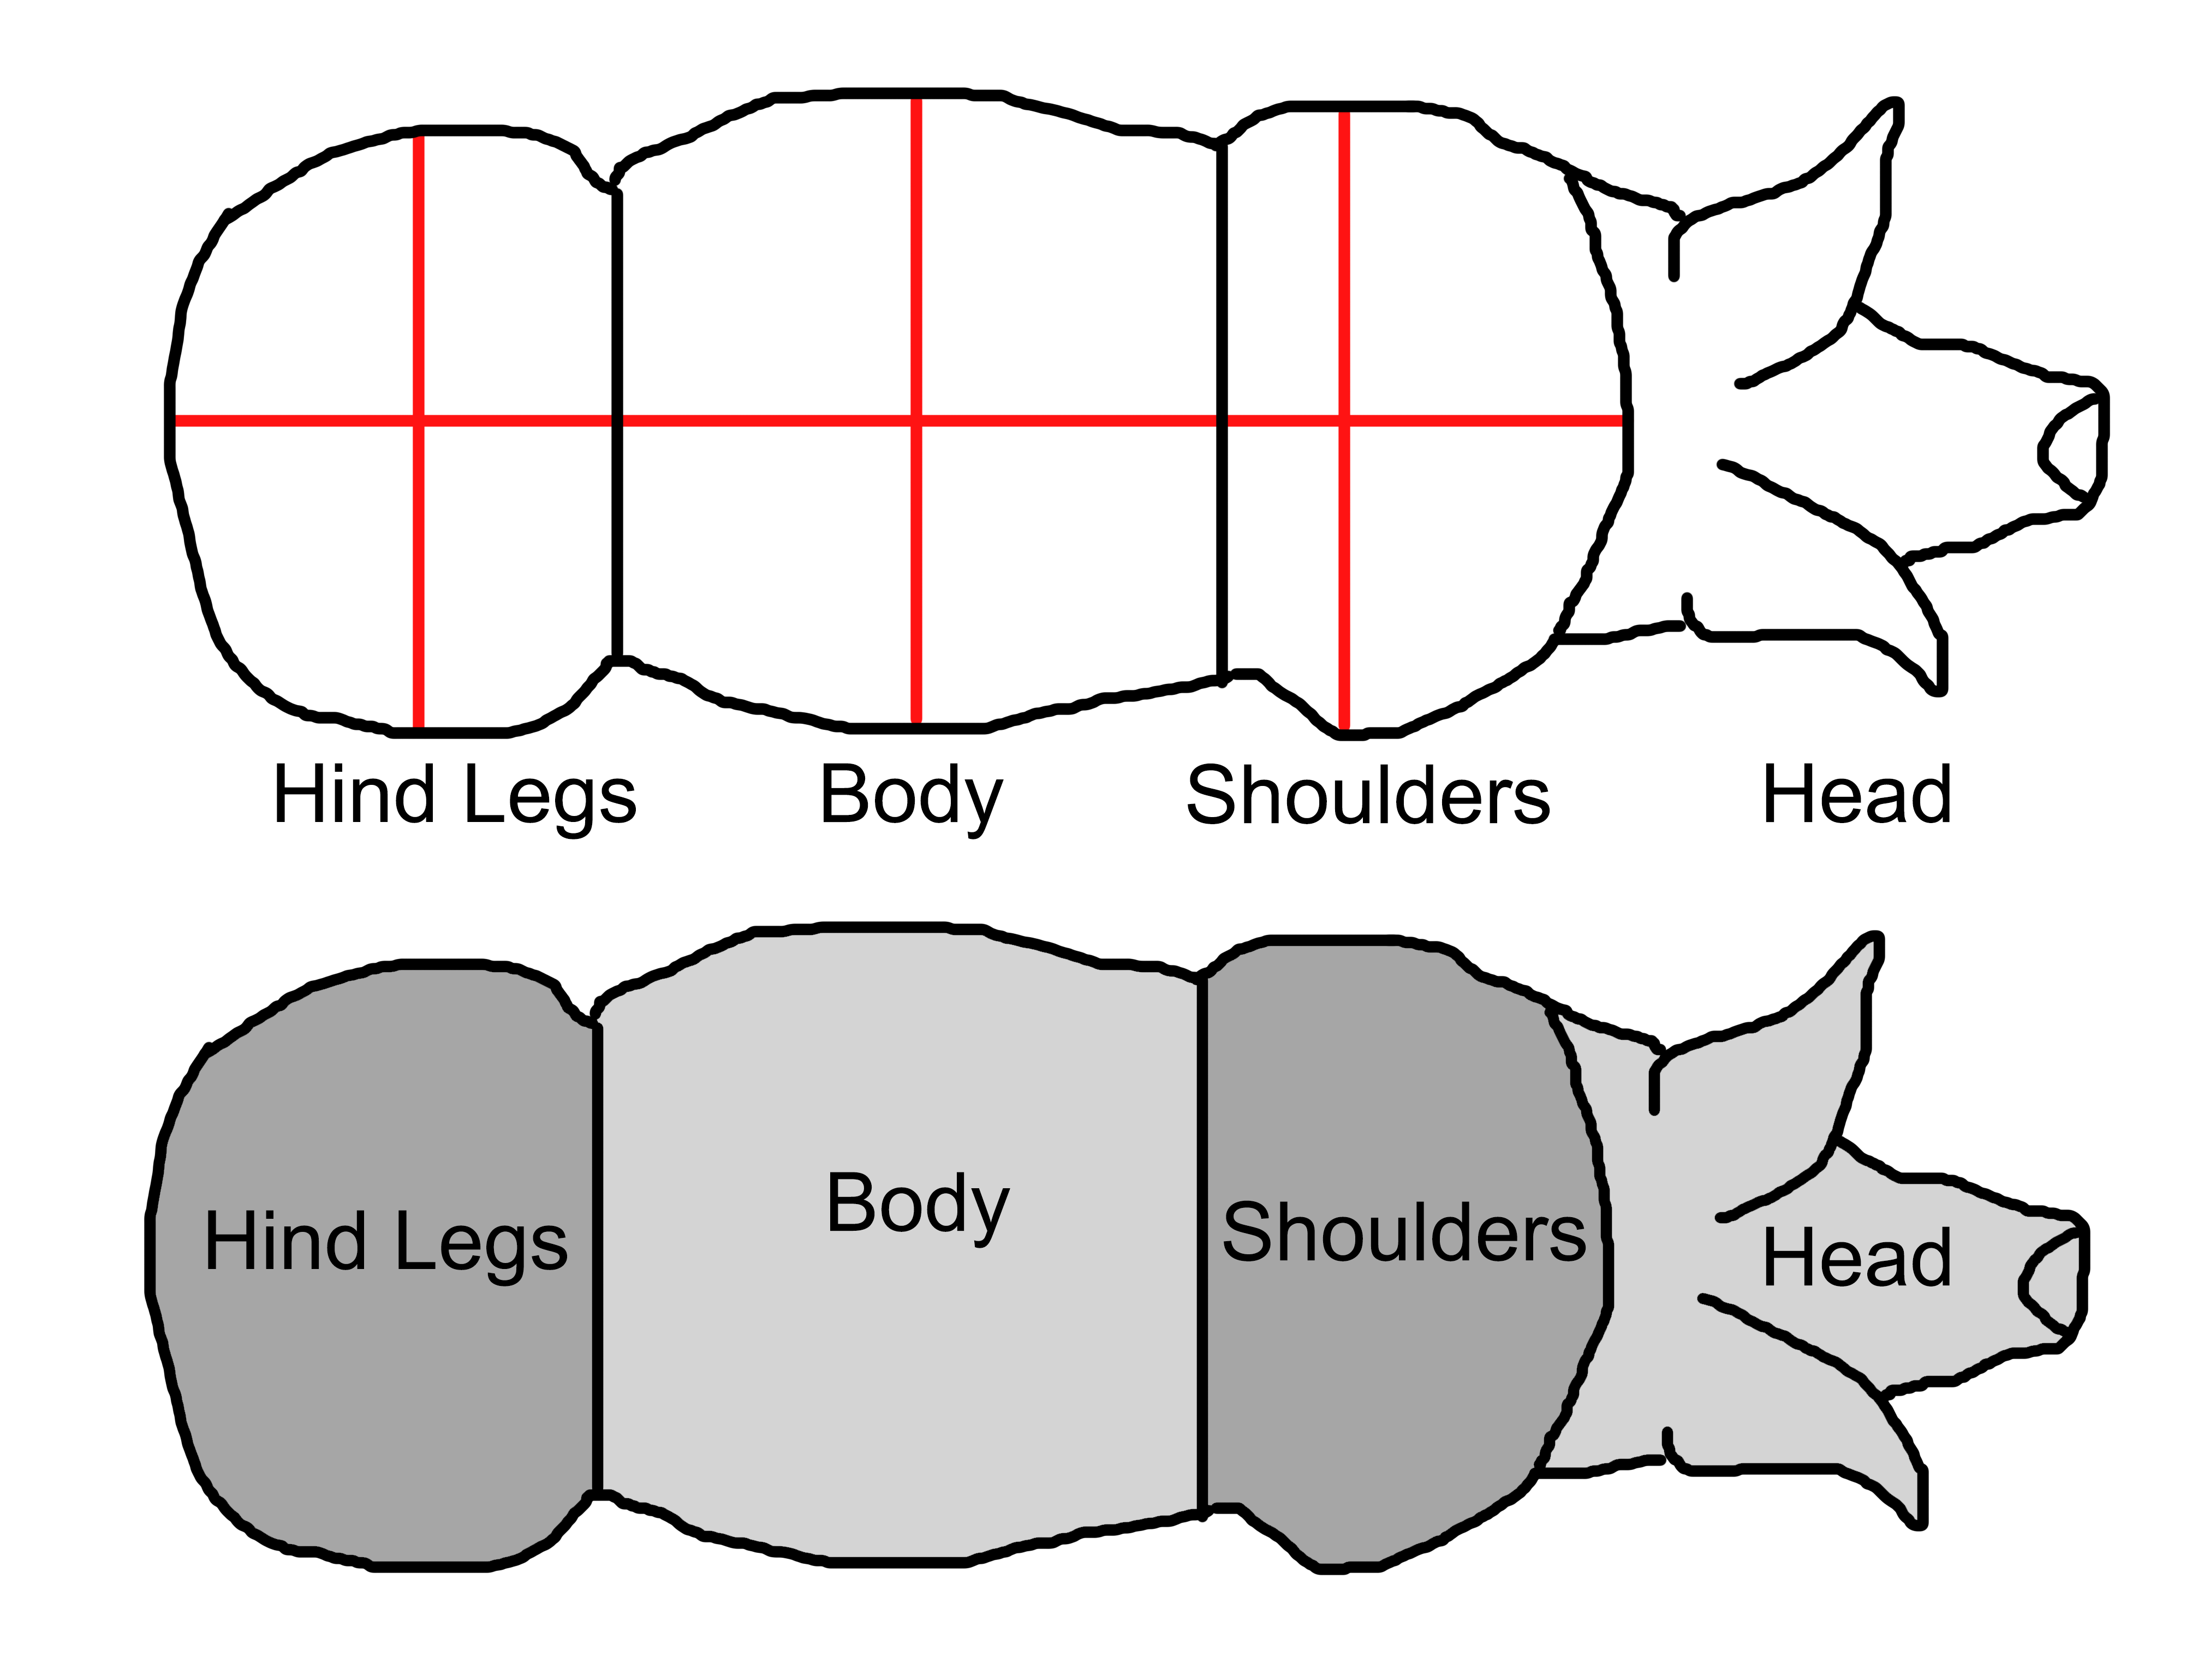
\includegraphics[height=0.4\textheight]{figures/Untitled-1 (1)}
	\caption{}
	\label{fig: Schematic representation of segmentation}
\end{figure}

Figure 5 shows a schematic representation of the segmentation of the pig. Following the segmentation process found in the study conducted by, the pig is segmented into four distinct parts: the hind legs, body, shoulder, and head. Using this segmentation framework, an algorithm will be developed to accurately divide the pig into these four areas. This is due to the difference in the pigs overall shape, allowing for more detailed data analysis and improved precision in data collection.

\section{Feature Extraction}
After segmentation, depth information is used to extract key features from the pig’s body. The Kinect sensor provides depth data $D(x,y)$, where the $x-axis$ and $y-axis$ represent the horizontal and vertical pixel coordinates of each point on the pig’s body, respectively. This data indicates the distance between the sensor and a specific point on the pig at a given pixel location $(x,y)$. Important features derived from this data include height, age, area, and gender.

\subsection{Height Extraction}
The height of the pig is determined by finding the maximum and minimum depth values within the segmented region. Let S(x,y) be the segmented mask of the pig. The height is calculated as:

\myequation{}
\begin{equation}
	x_{\text{highest}} = \max\{D(x, y) \mid (x, y) \in S(x, y)\}
\end{equation}

\myequation{}
\begin{equation}
	x_{\text{lowest}} = \min\{D(x, y) \mid (x, y) \in S(x, y)\}
\end{equation}

\myequation{}
\begin{equation}
	y_{\text{height}} = x_{\text{highest}} - x_{\text{lowest}}
\end{equation}

where $x_highest$ denotes the highest intensity and $x_lowest$ denotes the lowest intensity $S(x,y)$.

\subsection{Area Extraction}
The area occupied by the pig in the image is calculated by counting the number of pixels in the segmented region:

\myequation{}
\begin{equation}
	Area= \sum_{(x, y) \in S(x, y)} 1
\end{equation}

The area corresponds to the total number of pixels within the segmented pig’s contour, representing the surface area in the depth image.

\subsection{Gradient Information from Depth Data}
The depth gradient across the pig’s body provides additional insight into the pig’s shape. The gradient of the depth image D(x,y) can be computed using the finite difference approximation:

\myequation{}
\begin{equation}
	\delta(x,y)= (\frac{\partial}{\partial x} , \frac{\partial}{\partial y})
\end{equation}

This gradient gives us information about the slope of the pig’s body, which can be used to under more detailed features such as the body curvature and the slope of different anatomical regions The gradient magnitude can be used to detect regions of rapid change in depth, such as the transition from the pig’s back to its sides:

\myequation{}
\begin{equation}
	\left| \delta(x,y) \right| = \sqrt{\left( \frac{\partial}{\partial x} \right)^2 + \left( \frac{\partial}{\partial y} \right)^2}
\end{equation}

\section{Model Training}
In the model training phase, the extracted features will serve as inputs to various regression models aimed at estimating pig weight. We will explore several algorithms to identify the most accurate model for weight estimation: Linear Regression, Ridge Regression, Decision Trees, LightGBM, and XGBoost.

The analysis begins with linear regression, which models the linear relationship between features and weight, providing a straightforward baseline for comparison with more complex models (Mullainathan and Spiess, 2017). Ridge regression will be employed as an extension of linear regression, incorporating L2 regularization to mitigate overfitting, especially in cases of multicollinearity among input features. This approach enhances robustness against noisy data (Tikhonov, 1963).

Decision trees will also be utilized for their interpretability and ability to capture complex relationships within the data, though they require careful tuning to avoid overfitting (Breiman et al., 1986). LightGBM (Light Gradient Boosting Machine) is included for its efficiency and scalability with large datasets, utilizing a histogram-based learning approach to achieve faster training and improved accuracy (Ke et al., 2017). Additionally, XGBoost (Extreme Gradient Boosting) will be assessed for its high performance and optimizations for handling missing values and regularization, making it a leading choice in competitive machine-learning environments (Chen and Guestrin, 2016).
Model performance will be evaluated using metrics such as Mean Absolute Error (MAE) and Root Mean Squared Error (RMSE). MAE provides a clear measure of average error, while RMSE emphasizes larger errors, facilitating a comprehensive assessment of the model's accuracy (Willmott and Matsuura, 2005).

\section{Evaluation}
The trained models will undergo rigorous evaluation using a dedicated test dataset, comprising previously unseen data sampled randomly, which constitutes 30 percent of the overall dataset. This approach ensures that the evaluation accurately reflects the model's ability to generalize to new instances rather than merely memorizing the training data.
\subsection{Test Dataset}
By reserving 30 percent of the total dataset as the test dataset, we establish a method for assessing model performance. This test dataset will not have been exposed to the models during training, which is crucial for evaluating how well the models can predict weights on new data. The random sampling method ensures a representative distribution of weights and features, allowing for a fair assessment of the model's predictive capabilities.

\subsection{Performance Metrics}

To quantitatively evaluate the models, we will utilize the following performance metrics:
Mean Absolute Error (MAE). MAE calculates the average absolute difference between the actual values and the predicted values. It is a robust metric that does not penalize larger errors as heavily as MSE, making it more appropriate for interpreting the accuracy of regression models. The formula for MAE is:

\myequation{}
\begin{equation}
	MAE = \frac{1}{N} \sum_{t=1}^{N} \left| \hat{y_t} - y_t \right|
\end{equation}

The MAE metric gives a straightforward interpretation of error, as it expresses the average error directly in terms of the target variable (i.e., weight). It also equally weights all errors, making it a preferred choice for evaluating models that must perform reliably across a range of errors.

\subsection{Root Mean Squared Error (RMSE)}
RMSE provides a measure of how well the model's predictions match the actual data, expressed in the same units as the target variable. It is particularly useful as it penalizes larger errors more heavily, making it sensitive to outliers. The equation for RMSE is given by:

\myequation{}
\begin{equation}
	RMSE = \sqrt{\frac{1}{N} \sum_{t=1}^{N} \left( y_t - \hat{y_t} \right)^2}
\end{equation}

Where n is the number of observations in the test dataset, yi is the actual weight of the pig for the t-th observation, and yi is the predicted weight of the pig for the t-th observation.

\section{Testing Method}
An experimental setup will be used in this study to evaluate the accuracy and efficiency of the Kinect-based pig weight estimation system. The experimental setup will involve capturing depth images of pigs in a farming environment, followed by weight estimation using machine learning algorithms. The experimental setup allows systematic data collection and evaluation to verify the system’s performance compared to traditional weighing methods.

\section{Location}
The study will take place at a backyard pig-weaning farm located in El Salvador City, Misamis Oriental, Philippines. This particular farm was selected due to its favorable conditions and potential to serve as an ideal research site. To ensure reliable and consistent results, controlled conditions will be maintained throughout the study. The focus will be on Landrace pigs, which are known for their excellent growth and meat quality, with an average live weight ranging between 40 and 100 kg. This controlled environment will help ensure that any variables influencing the outcomes are carefully managed.

\section{Equipment}
The study utilizes a Microsoft Kinect V1 sensor, which will be mounted approximately 1.25 meters above the pigpen to capture a top-down view of each pig. The Kinect sensor is capable of providing depth images that are essential for measuring the pigs' physical dimensions. These depth images will be processed in real time by a computer system connected to the sensor. The system will run feature extraction algorithms designed to estimate the pigs' weight based on the data collected. To ensure accurate data capture, the pigpen will need to be free of obstructions around the pigs, as any occlusions could interfere with the depth imaging process. Additionally, consistent lighting will be maintained to reduce shadows and avoid image quality variations caused by fluctuating light conditions, both of which are crucial for producing reliable data. By addressing these factors, the study aims to provide precise and consistent measurements throughout the observation period.

\section{Data Collection}
The Kinect sensor will be positioned to capture depth images of each pig. Multiple images of each pig will be taken to account for posture variation. The system will discard low-quality images through an automatic image quality check. Using the captured images, the system will extract features such as body height, surface area, and volume from the depth data. These features will then be put into a pre-trained machine-learning model for weight estimation.. 
The Kinect sensor will be calibrated before the start of the data collection to ensure that the depth measurements are accurate and to compensate for the different lighting in the environment and the distance between the ground and the Kinect sensor. A reference weight for each pug will be recorded using a traditional weighing scale, which will use the accuracy of the Kinect-based system. The estimated weight from the depth images will be calculated automatically using the machine learning model through the system, which was trained using previously available data sets. The estimated values would then be compared to the reference weight values collected manually to assess the system's accuracy.

\section{Verification}

The verification process will involve comparing the weights estimated by the Kinect-based system with the actual weights recorded by the traditional weighing scale. A statistical analysis will be conducted where the Mean Absolute Error and the Root Mean Square Error will be calculated between the estimated and actual weights to quantify the system’s accuracy. Cross-validation will be done using a Test-Train split. The data set will be split into a 70 percent training set and a 30 percent testing set to ensure that the system is not overfitting and can generalize to new pigs. Different Machine learning models will then be tested to select the model with the best performance.